\problemname{Turnering}

\begin{tabular}{ccc}
  1. omgang & 2. omgang & 3. omgang\\[1ex]
  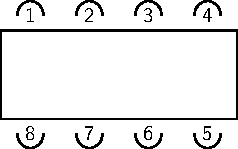
\includegraphics{img/turnering-img-1.pdf} &
  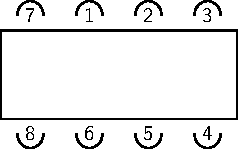
\includegraphics{img/turnering-img-2.pdf} &
  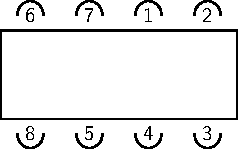
\includegraphics{img/turnering-img-3.pdf} 
\end{tabular}
\bigskip

Hvis man vil arrangere en alle-mod-alle-turnering, fx i skak, kan man benytte et rotationsprincip ved navn \emph{round robin}.
Det virker på den måde, at i første omgang møder spillerne hinanden som vist i ovenstående figur (vi antager, at antallet $n$ af spillere er lige.)
Efter første omgang flytter alle spillere sig ét skridt med uret -- bortset fra spilleren i nederste venstre hjørne, som bliver siddende.
(Man kan forestille sig, at princippets navn hentyder til, at man flytter sig »rundt om Robin«, som er den sidste spiller.) 
Med denne rotationsordning er det garanteret, at alle har mødt alle præcis én gang efter $n-1$ omgange.

Din opgave er at skrive et program, der beregner spiller-parringerne for en givet omgang.

\section*{Indlæsning}
En enkelt linje bestående af to heltal: antallet af spillere i turneringen (et lige tal $n$ mellem $2$ og $100$) og nummeret på omgangen (mellem $1$ og $n-1$).

\section*{Udskrift}

Programmet skal beskrive hvem der spiller mod hvem på $n/2$ linjer; hver linje har formatet \texttt{a-b}.
Rækkefølgen spiller ingen rolle.
